\documentclass[11pt]{article}

\usepackage{pablo}
\usepackage[a5paper,margin=1.8cm]{geometry}
\usepackage{multicol}

\pagestyle{empty}
\begin{document}

  \begin{center}
    {\large
      Devoir surveillé --- 1/2h --- Sujet A

      \textsc{Fonctions}
    }
  \end{center}

  \begin{exercice}[Droites --- 3 points]~

    \begin{multicols}{2}
      \begin{center}
        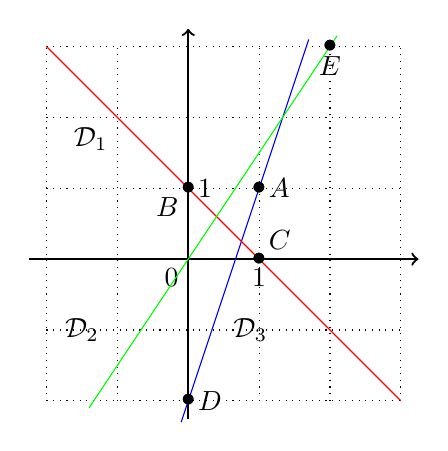
\begin{tikzpicture}[scale=0.9]
          \draw[color=black,step=1,dotted] (-2,-2) grid (3,3);
          \draw[thick,->] (-2.25,0) -- (3.25,0);
          \draw (1,0) node[below] {1};
          \draw[thick,->] (0,-2.25) -- (0,3.25);
          \draw (0,1) node[right] {1};
          \draw (0,0) node[below left] {0};
          \draw[color=blue,domain=-0.1:1.7] plot (\x,{3*\x-2});
          \draw[color=red,domain=-2:3] plot (\x,{-\x+1});
          \draw[color=green,domain=-1.4:2.1] plot (\x,{3*\x/2});
          \draw (-1,2) node[below left] {${\cal D}_1$};
          \draw (-1.5,-1) node[] {${\cal D}_2$};
          \draw (0.5,-1) node[right] {${\cal D}_3$};
          \draw (1,1) node{$\bullet$}node{$\bullet$}  node[right] {$A$};
          \draw (0,1) node{$\bullet$}node{$\bullet$}  node[below left] {$B$};
          \draw (1,0) node{$\bullet$}node{$\bullet$}  node[above right] {$C$};
          \draw (0,-2) node{$\bullet$}node{$\bullet$}  node[right] {$D$};
          \draw (2,3) node{$\bullet$}node{$\bullet$}  node[below] {$E$};
        \end{tikzpicture}
      \end{center}

      Les coordonnées des points $A$, $B$, $C$, $D$, et $E$ sont : $A(1,1)$, $B(0,1)$, $C(1,0)$, $D(0,-2)$, $E(2,3)$.

      Déterminer, par le calcul (sans lecture graphique), les équations des droites ${\cal D}_1$, ${\cal D}_2$ ${\cal D}_3$.
    \end{multicols}
  \end{exercice}

  \begin{exercice}[Problème --- 4 points] On se demande s'il est possible de construire le triangle rectangle suivant.

    \begin{center}
      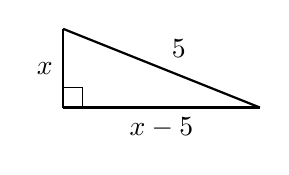
\begin{tikzpicture}[scale=0.5]
      \draw (0,0) rectangle (0.5,0.5);
      \draw[thick] (0,0) -- (5,0) node[midway,below] {$x-5$};
      \draw[thick] (5,0) -- (0,2) node[midway,above right] {$5$};
      \draw[thick] (0,2) -- (0,0) node[midway,left] {$x$};
    \end{tikzpicture}
    \end{center}
    \begin{enumerate}
      \item Montrer que $x$ vérifie : $x(2x-10)=0$.
      \item Résoudre cette équation.
      \item Interpréter les résultats : est-il possible de construire un tel triangle ?
    \end{enumerate}
  \end{exercice}

  \begin{exercice}[Équations produit et quotient --- 3 points]
    Résoudre les équations suivantes.

    \begin{multicols}{2}
    \begin{enumerate}[(a)]
      \item $(3x-1)(x+7)=0$
      \item $(x+1)^2(5x-1)=0$
      \item $\dfrac{7-3x}{3x}=0$
      \item $\dfrac{(3x-1)(x+7)}{x-2}=0$
      \item $\dfrac{2+x}{-2x-4}=0$
      \item $9x^2-6x+1=0$
      \item $x^2=-10x-25$
    \end{enumerate}
  \end{multicols}
  \end{exercice}

  \pagebreak
  \setcounter{exercice}{0}

  \begin{center}
    {\large
      Devoir surveillé --- 1/2h --- Sujet B

      \textsc{Fonctions}
    }
  \end{center}

  \begin{exercice}[Droites --- 3 points]~

    \begin{multicols}{2}
      \begin{center}
        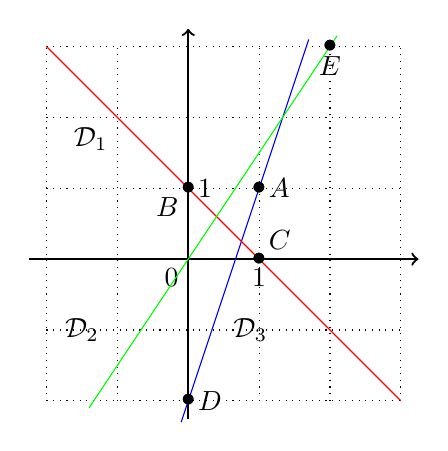
\begin{tikzpicture}[scale=0.9]
          \draw[color=black,step=1,dotted] (-2,-2) grid (3,3);
          \draw[thick,->] (-2.25,0) -- (3.25,0);
          \draw (1,0) node[below] {1};
          \draw[thick,->] (0,-2.25) -- (0,3.25);
          \draw (0,1) node[right] {1};
          \draw (0,0) node[below left] {0};
          \draw[color=blue,domain=-0.1:1.7] plot (\x,{3*\x-2});
          \draw[color=red,domain=-2:3] plot (\x,{-\x+1});
          \draw[color=green,domain=-1.4:2.1] plot (\x,{3*\x/2});
          \draw (-1,2) node[below left] {${\cal D}_1$};
          \draw (-1.5,-1) node[] {${\cal D}_2$};
          \draw (0.5,-1) node[right] {${\cal D}_3$};
          \draw (1,1) node{$\bullet$}node{$\bullet$}  node[right] {$A$};
          \draw (0,1) node{$\bullet$}node{$\bullet$}  node[below left] {$B$};
          \draw (1,0) node{$\bullet$}node{$\bullet$}  node[above right] {$C$};
          \draw (0,-2) node{$\bullet$}node{$\bullet$}  node[right] {$D$};
          \draw (2,3) node{$\bullet$}node{$\bullet$}  node[below] {$E$};
        \end{tikzpicture}
      \end{center}

      Les coordonnées des points $A$, $B$, $C$, $D$, et $E$ sont : $A(1,1)$, $B(0,1)$, $C(1,0)$, $D(0,-2)$, $E(2,3)$.

      Déterminer, par le calcul (sans lecture graphique), les équations des droites ${\cal D}_1$, ${\cal D}_2$ ${\cal D}_3$.
    \end{multicols}
  \end{exercice}

  \begin{exercice}[Problème --- 4 points] On se demande s'il est possible de construire le triangle rectangle suivant.

    \begin{center}
      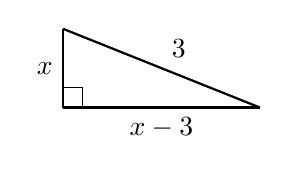
\begin{tikzpicture}[scale=0.5]
      \draw (0,0) rectangle (0.5,0.5);
      \draw[thick] (0,0) -- (5,0) node[midway,below] {$x-3$};
      \draw[thick] (5,0) -- (0,2) node[midway,above right] {$3$};
      \draw[thick] (0,2) -- (0,0) node[midway,left] {$x$};
    \end{tikzpicture}
    \end{center}
    \begin{enumerate}
      \item Montrer que $x$ vérifie : $x(2x-6)=0$.
      \item Résoudre cette équation.
      \item Interpréter les résultats : est-il possible de construire un tel triangle ?
    \end{enumerate}
  \end{exercice}
  \begin{exercice}[Équations produit et quotient --- 3 points]
    Résoudre les équations suivantes.

    \begin{multicols}{2}
    \begin{enumerate}[(a)]
      \item $(3x+1)(x-7)=0$
      \item $(x-1)^2(4x-1)=0$
      \item $\dfrac{6-3x}{2x}=0$
      \item $\dfrac{(3x+1)(x-7)}{x-3}=0$
      \item $\dfrac{3+x}{-2x-6}=0$
      \item $9x^2+6x+1=0$
      \item $x^2=+10x-25$
    \end{enumerate}
  \end{multicols}
  \end{exercice}


\end{document}
